%apdces.tex

\chapter{Mathematical Fundamentals}

\paragraph{Affine Transformation}
An Affine Transformation is one of the form
\[
y = Ax + b
\]
Where x,y,b are $N$ vectors, and A is an $N\times N$  matrix.  Such transformations perserve straight lines and include an offset ($b$) so that they can represent displacement as well as other types of linear transformations.


\section{Trigonometric Identities and Formulas}

\[
\sin^2(x)  + \cos^2(x) = 1
\]
\[
\sin(\pi/2-x) = \cos(x) \qquad \cos(\pi/2-x) = \sin(x)
\]
\[
sin(-x) = - sin(x) \qquad \cos(-x) = cos(x)
\]
\[
\sin(x+y) = \sin(x)\cos(y)+\cos(x)\sin(y) \qquad \cos(x+y) = \cos(x)\cos(y) -\sin(x)\sin(y)
\]

``Law of Cosines"
\begin{figure}
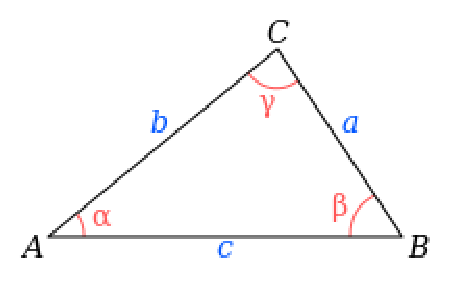
\includegraphics[width=2.0in]{figs_apdx/triangle.eps}
\caption{Source: wikipedia}
\end{figure}
\[
c^2 = a^2+b^2-2ab\cos(\gamma)
\]
\section{Euler Angle Sets}
\section{The Atan2 Function}

\newpage
\chapter{Linear Algebra Basics}\label{LinearAlgebraBasics}

Source: ``Introduction to Matrices and Determinants," F. Max Stein, 1967.

Assume $A$ is a square matrix.

Facts:

\begin{enumerate}
\item $A^{-1}$ exists if and only if
\[
\mathrm{det}[A] \ne 0
\]
if det$[A] = 0$, we say that $A$ is a $singular$ matrix and that its inverse does not exist.

\item The $rank$ of $A$ is the size of the largest square sub-matrix, $S$, for which
\[
\mathrm{det}[S] \ne 0
\]

\item If two rows or columns of $A$ are equal, or related by a constant, then det$[A]=0$.

\item Any singular matrix has at least one eigenvalue equal to zero.

\item If $A$ is non-singular, and $\lambda$ is an eigenvalue of $A$ corresponding to the eigenvector, $x$, then
\[
A^{-1}x = \lambda^{-1}x
\]

\item If $A$ is square, then $A$ and $A^T$ have the same eigenvalues.  I.e.
\[
Ax_i = \lambda_i x_i \qquad A^Ty_i = \lambda_i y_i
\]

\item If the $nxn$ matrix $A$ is of full rank (i.e. $r=n$) then the only solution to $Ax=0$ is the trivial one, $x=0$.

\item If $r<n$, then there are $n-r$ linearly independent (i.e. orthogonal) solutions
\[
x_j \qquad 1 < j < n-r
\]
for which $x_j\ne0$ and $Ax_j = 0$.

\end{enumerate}

\newpage
\section{Matrix Multiplication}
Conceptual Definition:
\begin{quotation}
A {\it matrix} is a mapping of a vector from one space to another which preserves straight lines.  The matrix thus represents a linear transformation.
\end{quotation}

Algebraic Definition:

If $A$ is a 3x3 matrix and $B$ is a 3x1 vector,

\[
AB =
\left[
\begin{array}{ccc}
a_{11}	& a_{12} & a_{13} \\
a_{21}  & a_{22} & a_{23} \\
a_{31}  & a_{32} & a_{33} \\
\end{array}
\right]
\times
\left[
\begin{array}{c}
b_1 \\ b_2 \\ b_3
\end{array}
\right]
= \left[
\begin{array}{c}
a_{11}b_1 + a_{12}b_2 + a_{13}b_3 \\
a_{21}b_1 + a_{22}b_3 + a_{23}b_3 \\
a_{31}b_1 + a_{32}b_3 + a_{33}b_3
\end{array}
\right]
\]

The rule is to multiply {\bf row by column} and add component wise.   This can also be written:

\[
AB_i = \sum_{j=1}^N  a_{ij}b_j
\]

For matrix - matrix multiplication, this becomes

\[
AC_{ij} = \sum_{m=1}^N  a_{im}c_{mj}
\]
where $C$ is a 3x3 matrix with components $c_{ij}$.

(Did you know that Albert Einstein invented the idea of dropping the $\sum$ and the subscripts to simpilify the notation of matrix multiplication?)
Putting it another way,

if

\[
A = \left [
\begin{array}{c}
a^T  \\ \alpha^T \\ \aleph^T
\end{array}
\right],
\mathrm{and} \qquad B = [b \quad \beta \quad \lambda],
\]
then
\[
AB = \left[
\begin{array}{ccc}
a \cdot b           &   a \cdot \beta             &  a  \cdot \lambda  \\
\alpha \cdot b      &   \alpha \cdot \beta        &  \alpha \cdot \lambda  \\
\aleph \cdot b      &   \aleph \cdot \beta        &  \aleph \cdot \lambda
\end{array}
\right]
\]
where $\cdot$ is the vector dot product.

\newpage
\section{Matrix Inverse}

\subsection{}
The inverse of a matrix $A$, $A^{-1}$ is most clearly defined by $AA^{-1} = I$.

We can find $A^{-1}$ by

\[
A^{-1} =  \frac{adj A}{det A} =
\left [
\begin{array}{ccc}
\frac{a_{11}}{|A|}      &   \frac{a_{12}}{|A|}      &   \frac{a_{13}}{|A|}     \\
 \dots                  &    \dots                  &  \dots                   \\
\dots                   &                           &  \frac{a_{ij}}{|A|}      \\
\end{array}
\right ]
\]

$adjA$ is a matrix of {\it cofactors} $A_{ij}$ of $A$ where
\[
A_{ij}  = (-1)^{n(j)}Det(A^{\_}(i,j))
\]
where $A^{\_}(i,j)$ is the matrix $A$ when row $i$ and col $j$ are removed and
\[
|A| = Det(A) = \sum_{\{j\}} (-1)^{n(j)} a_{1j_1}a_{2j_2}a_{3j_3}\dots a_{nj_n}
\]
where $\{j\}$ is the set of all permutations of the integers $i \dots n$, and $n(j)$ is the number of interchanges of the order of these permutations.


\subsection{}\label{2x2MatrixInverse}
For the case of a 2x2 matrix we have

\[
\begin{bmatrix} a_{11} & a_{12} \\ a_{21} & a_{22} \end{bmatrix} ^{-1} = \frac{1}{a_{11}a_{22}-a_{21}a{12}}
\begin{bmatrix} a_{22} & -a_{12} \\ -a_{21} & a_{11} \end{bmatrix}
\]






(This detail is included simply for completeness of the review.  For more information see your favorite Linear Algebra textbook.)




\newpage

\section{Interpretations of Matrix Vector Multiplication}
The following are helpful ways to think about the meaning or application of matrix-vector multiplication.
We will use a notation in which leading superscripts denote coordinate systems in which quantities are represented.  For example the
point $x$ may be represented by different coordinates in two different coordinate systems 1 and 2.    We denote these representations of
$x$ as $^1x, ^2x$.

\begin{enumerate}
  \item  Stretched Sheet

The matrix transformation $^2b = A ^1b$ can be visualized as the transformation of point $^1b$ on a rubber sheet which is
deformed to give a new point $^2b$.  Suppose a rubber sheet has three points $a, b, c$ printed on it and is streched as shown in Figure \ref{StretchedSheet}:

\begin{figure}
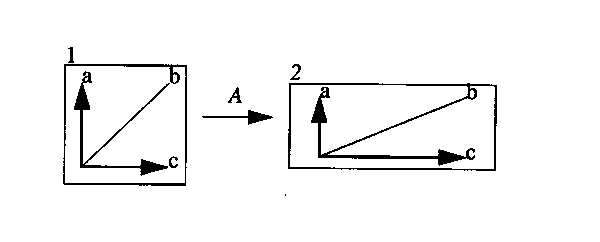
\includegraphics[width=3.5in]{figs11/00321.eps}
\caption{Matrix multiplication can be used to represent linear transformations such as the stretching of a rubber sheet.}\label{StretchedSheet}
\end{figure}

In this example, the stretching of the sheet can be described by the matrix $A$.   Looking at the figure we note that the vector $b$ is longer
after the stretch and points in a slightly different direction.   We also note that although $a$ and $c$ have had their lengths changed, they still point
in the same direction.   We can express this mathematically as
\[
^2a = \lambda_1a = A^1a
\]
and
\[
^2c = \lambda_2c = A^1c
\]
where $\lambda_1 $ and $\lambda_2 $ are scalar constants.   In other words, for this particular example, for certain vectors ($a,c$), the linear transformation
$A$ is eqivalent to multiplication by a constant, but not for general vectors such as $b$.
We call the scalars $\lambda_1$ and $\lambda_2$ the {\it eigenvalues} of $A$, and we call the vectors $a$ and $c$ the {\it eigenvectors} of $A$.

\item Rotation

We will cover this in considerable detail in Chapter XXXXXXX.

\item Magnification

Many aspects of optics including image magnification and some distortions such as keystoning can be represented by matrix vector multiplication.


\item Perspective Transformation

The mapping of 3D space to 2D such as is done in perspective drawings and camera imaging can be represented by matrices.


\end{enumerate}



\newpage
% ///////////////////////////////////////////////////////////////////////////////////////////////////////////////////

\section{Derivative of a Rotation Matrix}\label{derivativeofrotationmatrix}

In computing accelerations for dynamics we sometimes need the time derivative of a rotation matrix.
Consider a point rotated by angular velocity vector $\omega$.  The rotation represented by $\omega$ can also be represented by a time-varying rotation matrix,
$R(t)$.  Let's remember that every rotation matrix relates two frames.  In this case, a fixed frame, $F$, and the time-varying frame which we will call frame $R$, so that $R(t)$ could be written ${^F_RR(t)}$.    For now, assume that the angular velocity vector $\omega$ is known in $R(t)$ (somewhat unrealistic because $R(t)$ is constantly changing).

Using the classical definition of derivative:
\[
\frac{d}{dt} R(t)  = \lim_{\Delta t \to 0} \frac{R(t+\Delta t)P - R(t)}{\Delta t}
\]
\[
 = \lim_{\Delta t \to 0} \frac{R(t+\Delta t) - R(t)}{\Delta t}
\]
What is the difference between the two rotation matrices in the numerator?  The illustration below shows the two rotations, the vector $\omega$, and one of the three components of the difference: $\Delta t (\omega\times X)$.

\begin{center}
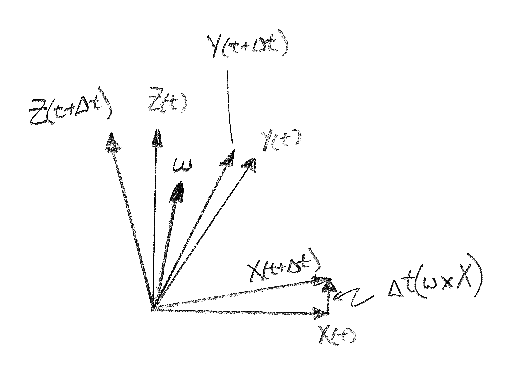
\includegraphics[width=3.5in]{figs_apdx/00917.eps}
\end{center}

Since each column of $R$ represents a unit vector of the frame, the difference of each column is the change introduced by the rotation $\omega$:

\[
 \frac{d}{dt} R(t) = \lim_{\Delta t \to 0} \frac{
     \bmat
         \Delta t\bmat\\ \omega\times X \\ \\ \emat & \Delta t\bmat \\ \omega \times Y \\ \\ \emat &  \Delta t\bmat \\  \omega \times Z \\ \\ \emat
     \emat
   }{\Delta t}
\]

\[
 = \lim_{\Delta t \to 0} \frac{
     \Delta t
     \bmat
         \omega\times \bmat 1\\0\\0 \emat & \omega\times\bmat 0\\1\\0 \emat &  \omega\times\bmat 0\\0\\1\emat
     \emat
   }{\Delta t}
\]

\[
         = \omega \times \bmat    1&0&0\\
                                  0&1&0\\
                                  0&0&1 \emat
\]
\[
\frac{d}{dt} R(t) = \dot{R} =
             \bmat       0   & -\omega_Z & \omega_Y   \\
                    \omega_Z &     0     & -\omega_X  \\
                   -\omega_Y & \omega_X  &    0       \emat
\]


What we have found now is that we can express the time derivative of a rotation matrix as a skew-symmetrix matrix as a function of the components of the angular velocity vector $\omega$.
There is only one problem: in this expansion, we assumed that the vector $\omega$ was known in the time varying frame, $R$.  Instead we want an expression with the known angular velocity: $^F\omega$.

Let's apply our result to mapping a point to a time varying rotated frame:
\[
 \dot{R}P =
             \bmat       0   & -\omega_Z & \omega_Y   \\
                    \omega_Z &     0     & -\omega_X  \\
                   -\omega_Y & \omega_X  &    0       \emat  P
\]
\[
\dot{R}P = ^R\omega\times P
\]
where we applied the matrix interpretation of the cross product.

To fix the problem that $^R\omega$ is not known, we note that if we rotate $\omega$ from $F$ to $R$ we can express $^R\omega$ in terms of the known $^F\omega$:
\[
\dot{R}P = \;{^R_FR}\; ^F\omega\times P
\]

by application of a cross-product property:
\[
\dot{R}P = \; ^F\omega\times {^F_RR}\; P
\]
Thus when it appears in a matrix-vector or (by extension) matrix-matrix multiplication, we can write the derivative of the rotation matrix $R$ as
\[
\dot{R} = \omega \times R \qquad \mathrm{or} \qquad \bmat       0   & -\omega_Z & \omega_Y   \\
                  \omega_Z &     0     & -\omega_X  \\
                 -\omega_Y & \omega_X  &    0       \emat R
\]





\newpage

\section{Inspiration}
\begin{quotation}
The engineer generalizes the 1,2, or 3 dimensional problem of the physicist into k dimensions."
\end{quotation}
Gabriel Kron, ``Tensor Analysis of Networks," 1938.







% ///////////////////////////////////////////////////////////////////////////////////////////////////////////////////
% /////////
% //    Appendix Section:
% //
\newpage
\chapter{Comparison of Rotation Representations}

In Chapter 2 we covered several methods to represent the rotation of rigid objects and end  effectors.  It is natural to ask which of these is ``best" to use in writing analysis and writing software to control robot manipulators.  We have covered the following representations:

\begin{itemize}
  \item 3-parameter systems:  roll-pitch-yaw,  ZYX Euler angles,  etc.
  \item Equivalent angle-axis
  \item Quaternions
  \item Rotation Matrices
\end{itemize}

In choosing a ``best" representation, we must define a set of criteria.


\begin{itemize}
  \item Compatibility with dynamics, sensor processing, and control equations
  \item Numerical roundoff and normalization issues.
  \item Numerical singularities
  \item Memory Usage
  \item Computational efficiency
\end{itemize}

\paragraph{Compatibility}
This and other books have reviewed several widely used computations for forward and inverse kinematics, Jacobian matrices, dynamics, joint-space and cartesian space trajectory planning, and many others.   Most of these algorithms stick to one or two of the representations we have reviewed.   Robust, well known algorithms for each computation are not widely available for each representation.  Thus we must evaluate the choice of representation according to how well it can be used in the various computations needed to control and operate a robot manipulator.

\paragraph{Numerical Issues}
Each method has strengths and weaknesses when they are implemented in computer software.

\paragraph{Computational and Memory Efficiency}
In considering all of these factors, we must also consider Moore's Law which reduces the cost of computational resources by about two orders of magnitude each time a new robotics textbook comes out.   Moore's well known Law states that the available computation per unit cost increases by a factor of 2 every 1.5 years.
Specifically, since the 1980's (30 years as of this writing) if $C_{1982}$ is the amount of computing power avialable in 1982,
\[
C_{2012} = 2^{(30/1.5)}C_{1982} = 1048576C_{1982}
\]
In other words, computer power today is 1 Million times greater than in the 1980's!
 Since the kinematic complexity of robot manipulators grows much more slowly than Moore's Law, at the time of this writing computational efficiency and memory usage differences between the methods are essentially insignificant for computational implementation of the kinematic and dynamic models of practical manipulators.

We are thus left with only the first three criteria,
 Compatibility with dynamics, sensor processing, and control equations.
 Numerical roundoff and normalization issues,  and
 Singularities.


\section{Comparison of Rotation Representations}
In this section we will evaluate each rotation representation in the context of each of the criteria described above.

\subsection{Compatibility with Inverse Kinematics, dynamics, sensor processing, and control equations}


\paragraph{Dynamics}

Dynamic equations are commonly computed by either the recursive Newton Euler method, or the Lagrange method.
When derived using the Lagrange method, rotational velocities are used to compute  kinetic and potential energy.  In most references, these computations are done with respect to the manipulator joint variables ($\theta_i, d_j$, most commonly refered to as $q_k$) and so do not require a choice of reprsentation for link angular velocity or acceleration.   Thus the following systems will be assessed for the Newton-Euler method.



\begin{itemize}
  \item 3-parameter systems:  roll-pitch-yaw,  ZYX Euler angles,  etc.



When orientation is expressed in one of the three-parameter systems, rate of change in orientation is most often expressed as as angular velocity, and angular acceleration vectors defined as:

\[
\omega = \begin{bmatrix} \omega_x, \omega_y, \omega_z \end{bmatrix}
\qquad
\dot{\omega} = \frac{d}{dt}\omega =  \begin{bmatrix} \dot{\omega}_x, \dot{\omega}_y, \dot{\omega}_z \end{bmatrix}
\]


When dynamics are computed using the Recursive Newton-Euler method,
$\omega, \dot{\omega}$ are commonly used.  But singularities are a potential problem.
% Computation of link torques (Euler's equation) is somewhat of a special case however since relative angular velocity between links is limited to z components (?????? makes sense ????)





  \item Equivalent angle-axis

The dynamic equations are rarely expressed in Equvalent angle-axis form.


  \item Quaternions

Quaternions have historically been used in rigid body dynamics.   Euler's equation for rotational motion can be written in quaternion form\footnote{"Rigid Body Dynamics using Euler's equations, Runge-Kutta and quaternions," Indrek Mandre, 2008.} as
\[
\ddot{q}(t) = \dot{q}q^*\dot{q}+ \frac12q\left[I^{-1}(\tau(t,q,\dot{q})-4(q^*\dot{q})\times(I(q*\dot{q})))\right]
\]
where $I$ is the rigid body intertia tensor, and $\tau(t,q,\dot{q})$ is the sum of external, elastic, and viscous torques on the rigid body.  This equation can be integrated twice to get the quaternion, $q(t)$, specifying the orientation of the rigid body with time.



  \item Rotation Matrices

Rotation matrices by themselves are used in dynamic equations for coordinate transformations, but are not used to represent angular velocities or accelerations.


\end{itemize}





\section{Roundoff and Normalization}

Computers represent floating point numbers with finite precision.  In some computations, entities like rotation matrices and quaternions are successively multiplied over and over.  In such cases, roundoff errors can accumulate.  One difficulty with such accumulation of error is that unit quaternions and rotation matrices can loose properties such as normalization or orthonormality.

Numerical procedures exist to correct these errors called normalization or re-normalization procedures.  They can be performed every so often as a precaution against loss of normality constraints.  Renormalization does not guarantee lack of error however.   Although the cost of renormalization varies considerably, we shall also consider it insignificant for computations covered in this book.


Numerical issues can arise in multiple different ways.  For specificity, we consider here the process of frequently updating an orientation reference by an increment of orientation.

\begin{itemize}

  \item 3-parameter systems:  roll-pitch-yaw,  ZYX Euler angles,  etc.

  Three parameter representations can be updated by addition if about an unchanging axis which causes few numerical issues.   If the axis of rotation is changing, this representation becomes difficult to update.

  \item Equivalent angle-axis

   With respect to numerical issues, equivalent angle-axis can be thought of as a version of quaternions (below).

  \item Quaternions

Quaternions are updated by multiplication (Equation (\ref{quaternionproduct})) and are subject to cumulative roundoff errors which can lead to loss of normalization.  A quaternion can be re-normalized similarly to a vector:
If $q = [w,x,y,z]$, the normalized version, $\hat{q}$ is
\[
\hat{q} = \frac{q}{\sqrt{w^2 + x^2 + y^2 + z^2}}
\]

  \item Rotation Matrices

Rotation matrices gradually loose their orthonormality due to build up of roundff errors which accumulate from multiple computations.   As a result, a matrix which should represent the product of hundreds or thousands of rotations may, due to accumulated roundoff errors, represent a dilation in addition to rotation.
Renormalization of a rotation matrix is more involved than for a vector because the columns and rows must be orthogonalized as well as re-set to unit magitude.

The cure for this is to periodically apply a renormalization algorithm to the matrix $\tilde{R}$ which is in need of renormalization.  In one such method, use singular value decomposition to convert $\tilde{R}$ into three components:

\[
U\Sigma V^* = \mathrm{SVD}(\tilde{R})
\]
Then the renormalized matrix $\hat{R}$ is
\[
\hat{R} = U\begin{bmatrix} 1&0&0 \\0&1&0\\0&0&1 \end{bmatrix}V^*
\]
Although SVD computation is $O(n^4)$, $3^4=81$ computations must be considered a reasonable number with current and future available computing power.



\end{itemize}





\section{Singularities}

We consider here the difference between algorithmic singularities and mechanical singularies.   A robot has a mechanical singularity whenever it occupies a joint configuration which causes its Jacobian matrix to loose rank.  This corresponds to a physical ``lock-up" of the mechanism and a loss of at least one direction of motion freedom.  On the other hand, the equations which convert a rotation matrix to, for example, roll-pitch-yaw angles, have a singularity whenever xxxxx(cite to chapter 2)xxxxx.    This is independent of the actual mechanism state and depends on the chosen coordinate system --- an algorithmic singularity.

\begin{itemize}
  \item 3-parameter systems:  roll-pitch-yaw,  ZYX Euler angles,  etc.

As we saw in Chapter 2, each 3-parameter system has a specific orientation containing an algorithmic singularity.  Algorithms which use a 3-parameter approach must be careful to check for this singularity or find guarantees that the computations stay away from the singularty in the chosen coordinate system and application.

  \item Equivalent angle-axis

Equivalent angle-axis is defined for any finite rotation, but can be considered singular when the rotation is zero, corresponding to the case where
\[
{^A_BR} = \begin{bmatrix}  1&0&0 \\0&1&0\\0&0&1\end{bmatrix}
\]
This singularity may be relatively benign in many applications because 1) it is independent of the chosen coordinate system and 2) it corresponds to a null rotation.


  \item Quaternions

Quaternions have the same singularity situation as Equivalent angle-axis


  \item Rotation Matrices

Rotation matrices have no singularities.  They are well defined (have determinant = 1) for any orienation in any coordinate system.

\end{itemize}



\newpage
\begin{thebibliography}{1}

\bibitem{x} The following books have been invaluable in preparation of these notes.


\bibitem{springerhandbook}
B.~Siciliano and O.~Khatib, editors.
\newblock {\em Springer Handbook of Robotics}.
\newblock Springer, Berlin, Heidelberg, 2008.

\bibitem{paul1981robot}
Richard~P Paul.
\newblock {\em Robot manipulators: mathematics, programming, and control: the
  computer control of robot manipulators}.
\newblock the MIT Press, 1981.

\bibitem{asada1986robot}
Haruhiko Asada and Jean-Jacques~E Slotine.
\newblock {\em Robot analysis and control}.
\newblock J. Wiley New York, NY, 1986.

\bibitem{nakamura1990advanced}
Yoshihiko Nakamura.
\newblock {\em Advanced robotics: redundancy and optimization}.
\newblock Addison-Wesley Longman Publishing Co., Inc., 1990.

\bibitem{yoshikawa1990foundations}
Tsuneo Yoshikawa.
\newblock {\em Foundations of robotics: analysis and control}.
\newblock The MIT Press, 1990.

\bibitem{Craig86}
J.~Craig.
\newblock {\em Introduction to Robotics: Mechanics and Control}.
\newblock Addison Wesley, 1986.

\bibitem{jazar2007theory}
Reza~N Jazar.
\newblock {\em Theory of applied robotics: kinematics, dynamics, and control}.
\newblock Springerverlag Us, 2007.

\end{thebibliography}










% \chapter{Inertia Tensor and Transformations of the Inertia Tensor}
%
%
% \chapter{Singular Value Decomposition}
%
% \chapter{Matrix Pseudo Inverse}